\documentclass{standalone}
\usepackage{tikz}
\usetikzlibrary{patterns, positioning}
\usepackage[sfdefault]{ClearSans} %% option 'sfdefault' activates Clear Sans as the default text font
\usepackage[T1]{fontenc}

\begin{document}
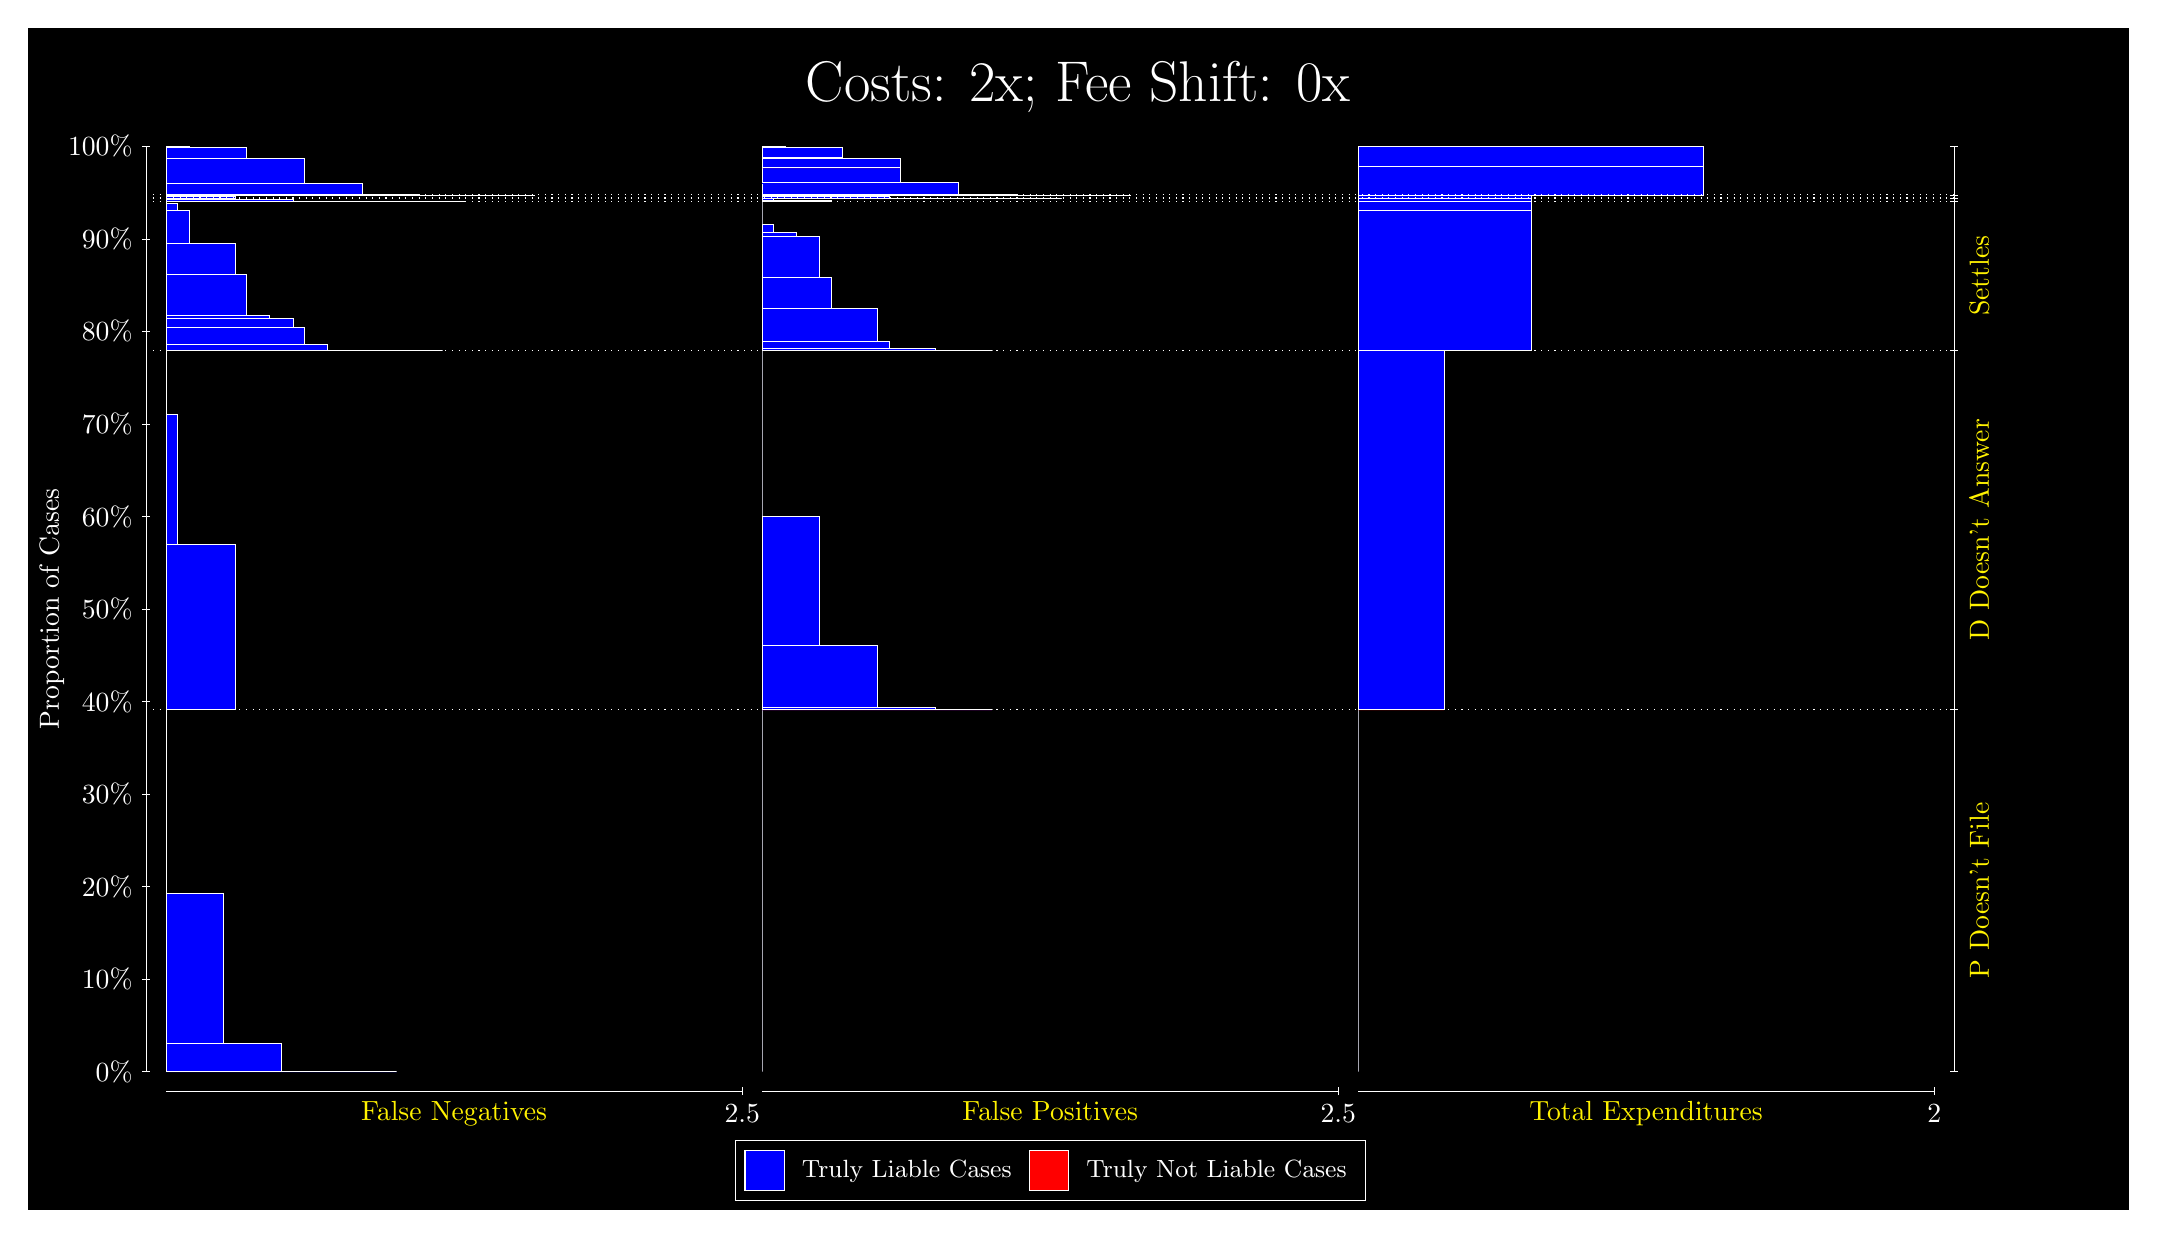
\begin{tikzpicture}
\draw[fill=black] (0,0) rectangle (26.667,15);
\draw[text=white] (0,13.5) rectangle (26.667,15) node[midway] {\huge Costs: 2x; Fee Shift: 0x};
\draw[white, very thin] (1.5,1.75) -- (1.5,13.5);
\node[rotate=90, text=white, anchor=center] at (0.3, 7.625) {Proportion of Cases};
\draw[white, very thin] (1.45,1.75) -- (1.55,1.75);
\node[text=white, anchor=east] at (1.45, 1.75) {0\%};
\draw[white, very thin] (1.45,2.925) -- (1.55,2.925);
\node[text=white, anchor=east] at (1.45, 2.925) {10\%};
\draw[white, very thin] (1.45,4.1) -- (1.55,4.1);
\node[text=white, anchor=east] at (1.45, 4.1) {20\%};
\draw[white, very thin] (1.45,5.275) -- (1.55,5.275);
\node[text=white, anchor=east] at (1.45, 5.275) {30\%};
\draw[white, very thin] (1.45,6.45) -- (1.55,6.45);
\node[text=white, anchor=east] at (1.45, 6.45) {40\%};
\draw[white, very thin] (1.45,7.625) -- (1.55,7.625);
\node[text=white, anchor=east] at (1.45, 7.625) {50\%};
\draw[white, very thin] (1.45,8.8) -- (1.55,8.8);
\node[text=white, anchor=east] at (1.45, 8.8) {60\%};
\draw[white, very thin] (1.45,9.975) -- (1.55,9.975);
\node[text=white, anchor=east] at (1.45, 9.975) {70\%};
\draw[white, very thin] (1.45,11.15) -- (1.55,11.15);
\node[text=white, anchor=east] at (1.45, 11.15) {80\%};
\draw[white, very thin] (1.45,12.325) -- (1.55,12.325);
\node[text=white, anchor=east] at (1.45, 12.325) {90\%};
\draw[white, very thin] (1.45,13.5) -- (1.55,13.5);
\node[text=white, anchor=east] at (1.45, 13.5) {100\%};

\draw[white, very thin] (24.457,1.75) -- (24.457,13.5);
\draw[white, very thin] (24.407,1.75) -- (24.507,1.75);
\node[anchor=west] at (24.407, 1.75) {};
\draw[white, very thin] (24.407,6.3462) -- (24.507,6.3462);
\node[anchor=west] at (24.407, 6.3462) {};
\draw[white, very thin] (24.407,10.912) -- (24.507,10.912);
\node[anchor=west] at (24.407, 10.912) {};
\draw[white, very thin] (24.407,12.801) -- (24.507,12.801);
\node[anchor=west] at (24.407, 12.801) {};
\draw[white, very thin] (24.407,12.844) -- (24.507,12.844);
\node[anchor=west] at (24.407, 12.844) {};
\draw[white, very thin] (24.407,12.884) -- (24.507,12.884);
\node[anchor=west] at (24.407, 12.884) {};
\draw[white, very thin] (24.407,13.5) -- (24.507,13.5);
\node[anchor=west] at (24.407, 13.5) {};

\draw[white, very thin, fill=blue] (1.75,1.75) rectangle (4.6775,1.75);
\draw[white, very thin, fill=blue] (1.75,1.75) rectangle (3.9457,1.753);
\draw[white, very thin, fill=blue] (1.75,1.753) rectangle (3.2138,2.1102);
\draw[white, very thin, fill=blue] (1.75,2.1102) rectangle (2.4819,4.0187);
\draw[white, very thin, fill=red] (1.75,4.0187) rectangle (1.75,4.0187);
\draw[white, very thin, fill=blue] (1.75,4.0187) rectangle (1.75,6.3462);
\draw[white, very thin, fill=blue] (1.75,6.3462) rectangle (2.6283,8.4509);
\draw[white, very thin, fill=blue] (1.75,8.4509) rectangle (1.8964,10.091);
\draw[white, very thin, fill=red] (1.75,10.091) rectangle (1.75,10.091);
\draw[white, very thin, fill=blue] (1.75,10.091) rectangle (1.75,10.912);
\draw[white, very thin, fill=blue] (1.75,10.912) rectangle (5.2631,10.912);
\draw[white, very thin, fill=blue] (1.75,10.912) rectangle (4.5312,10.914);
\draw[white, very thin, fill=blue] (1.75,10.914) rectangle (4.092,10.916);
\draw[white, very thin, fill=blue] (1.75,10.916) rectangle (3.7993,10.98);
\draw[white, very thin, fill=blue] (1.75,10.98) rectangle (3.5065,11.205);
\draw[white, very thin, fill=blue] (1.75,11.205) rectangle (3.3602,11.31);
\draw[white, very thin, fill=blue] (1.75,11.31) rectangle (3.0674,11.358);
\draw[white, very thin, fill=blue] (1.75,11.358) rectangle (2.7746,11.874);
\draw[white, very thin, fill=blue] (1.75,11.874) rectangle (2.6283,12.268);
\draw[white, very thin, fill=blue] (1.75,12.268) rectangle (2.3355,12.269);
\draw[white, very thin, fill=blue] (1.75,12.269) rectangle (2.0428,12.684);
\draw[white, very thin, fill=blue] (1.75,12.684) rectangle (1.8964,12.783);
\draw[white, very thin, fill=red] (1.75,12.783) rectangle (1.75,12.783);
\draw[white, very thin, fill=blue] (1.75,12.783) rectangle (1.75,12.801);
\draw[white, very thin, fill=blue] (1.75,12.801) rectangle (5.5558,12.801);
\draw[white, very thin, fill=blue] (1.75,12.801) rectangle (4.8239,12.801);
\draw[white, very thin, fill=blue] (1.75,12.801) rectangle (4.092,12.802);
\draw[white, very thin, fill=blue] (1.75,12.802) rectangle (3.3602,12.828);
\draw[white, very thin, fill=blue] (1.75,12.828) rectangle (2.6283,12.844);
\draw[white, very thin, fill=red] (1.75,12.844) rectangle (1.75,12.844);
\draw[white, very thin, fill=blue] (1.75,12.844) rectangle (2.6283,12.86);
\draw[white, very thin, fill=blue] (1.75,12.86) rectangle (1.8964,12.883);
\draw[white, very thin, fill=red] (1.75,12.883) rectangle (1.75,12.883);
\draw[white, very thin, fill=blue] (1.75,12.883) rectangle (1.75,12.884);
\draw[white, very thin, fill=blue] (1.75,12.884) rectangle (6.4341,12.884);
\draw[white, very thin, fill=blue] (1.75,12.884) rectangle (5.7022,12.884);
\draw[white, very thin, fill=blue] (1.75,12.884) rectangle (4.9703,12.892);
\draw[white, very thin, fill=blue] (1.75,12.892) rectangle (4.2384,13.035);
\draw[white, very thin, fill=blue] (1.75,13.035) rectangle (3.5065,13.344);
\draw[white, very thin, fill=blue] (1.75,13.344) rectangle (2.7746,13.487);
\draw[white, very thin, fill=blue] (1.75,13.487) rectangle (2.0428,13.5);
\draw[white, very thin, fill=red] (1.75,13.5) rectangle (1.75,13.5);
\draw[white, very thin, fill=blue] (1.75,13.5) rectangle (1.75,13.5);
\draw[white, very thin, fill=red] (9.3189,1.75) rectangle (9.3189,1.75);
\draw[white, very thin, fill=blue] (9.3189,1.75) rectangle (9.3189,6.3462);
\draw[white, very thin, fill=red] (9.3189,6.3462) rectangle (12.246,6.3462);
\draw[white, very thin, fill=blue] (9.3189,6.3462) rectangle (12.246,6.3462);
\draw[white, very thin, fill=blue] (9.3189,6.3462) rectangle (11.515,6.3716);
\draw[white, very thin, fill=blue] (9.3189,6.3716) rectangle (10.783,7.1678);
\draw[white, very thin, fill=blue] (9.3189,7.1678) rectangle (10.051,8.8076);
\draw[white, very thin, fill=blue] (9.3189,8.8076) rectangle (9.3189,10.912);
\draw[white, very thin, fill=red] (9.3189,10.912) rectangle (12.246,10.912);
\draw[white, very thin, fill=blue] (9.3189,10.912) rectangle (12.246,10.912);
\draw[white, very thin, fill=red] (9.3189,10.912) rectangle (11.661,10.912);
\draw[white, very thin, fill=blue] (9.3189,10.912) rectangle (11.661,10.915);
\draw[white, very thin, fill=blue] (9.3189,10.915) rectangle (11.515,10.93);
\draw[white, very thin, fill=blue] (9.3189,10.93) rectangle (10.929,11.029);
\draw[white, very thin, fill=blue] (9.3189,11.029) rectangle (10.783,11.444);
\draw[white, very thin, fill=red] (9.3189,11.444) rectangle (10.49,11.444);
\draw[white, very thin, fill=blue] (9.3189,11.444) rectangle (10.49,11.445);
\draw[white, very thin, fill=blue] (9.3189,11.445) rectangle (10.197,11.839);
\draw[white, very thin, fill=blue] (9.3189,11.839) rectangle (10.051,12.355);
\draw[white, very thin, fill=blue] (9.3189,12.355) rectangle (9.758,12.403);
\draw[white, very thin, fill=blue] (9.3189,12.403) rectangle (9.4652,12.508);
\draw[white, very thin, fill=blue] (9.3189,12.508) rectangle (9.3189,12.801);
\draw[white, very thin, fill=red] (9.3189,12.801) rectangle (10.197,12.801);
\draw[white, very thin, fill=blue] (9.3189,12.801) rectangle (10.197,12.817);
\draw[white, very thin, fill=blue] (9.3189,12.817) rectangle (9.4652,12.843);
\draw[white, very thin, fill=blue] (9.3189,12.843) rectangle (9.3189,12.844);
\draw[white, very thin, fill=red] (9.3189,12.844) rectangle (13.125,12.844);
\draw[white, very thin, fill=blue] (9.3189,12.844) rectangle (13.125,12.844);
\draw[white, very thin, fill=blue] (9.3189,12.844) rectangle (12.393,12.844);
\draw[white, very thin, fill=blue] (9.3189,12.844) rectangle (11.661,12.845);
\draw[white, very thin, fill=blue] (9.3189,12.845) rectangle (10.929,12.868);
\draw[white, very thin, fill=blue] (9.3189,12.868) rectangle (10.197,12.884);
\draw[white, very thin, fill=red] (9.3189,12.884) rectangle (14.003,12.884);
\draw[white, very thin, fill=blue] (9.3189,12.884) rectangle (14.003,12.884);
\draw[white, very thin, fill=red] (9.3189,12.884) rectangle (13.271,12.884);
\draw[white, very thin, fill=blue] (9.3189,12.884) rectangle (13.271,12.884);
\draw[white, very thin, fill=red] (9.3189,12.884) rectangle (12.539,12.884);
\draw[white, very thin, fill=blue] (9.3189,12.884) rectangle (12.539,12.896);
\draw[white, very thin, fill=blue] (9.3189,12.896) rectangle (11.807,13.039);
\draw[white, very thin, fill=red] (9.3189,13.039) rectangle (11.807,13.039);
\draw[white, very thin, fill=blue] (9.3189,13.039) rectangle (11.807,13.04);
\draw[white, very thin, fill=blue] (9.3189,13.04) rectangle (11.075,13.231);
\draw[white, very thin, fill=red] (9.3189,13.231) rectangle (11.075,13.231);
\draw[white, very thin, fill=blue] (9.3189,13.231) rectangle (11.075,13.349);
\draw[white, very thin, fill=blue] (9.3189,13.349) rectangle (10.344,13.364);
\draw[white, very thin, fill=blue] (9.3189,13.364) rectangle (10.344,13.491);
\draw[white, very thin, fill=blue] (9.3189,13.491) rectangle (9.6116,13.491);
\draw[white, very thin, fill=blue] (9.3189,13.491) rectangle (9.6116,13.5);
\draw[white, very thin, fill=blue] (9.3189,13.5) rectangle (9.3189,13.5);
\draw[white, very thin, fill=red] (16.888,1.75) rectangle (16.888,1.75);
\draw[white, very thin, fill=blue] (16.888,1.75) rectangle (16.888,6.3462);
\draw[white, very thin, fill=red] (16.888,6.3462) rectangle (17.986,6.3462);
\draw[white, very thin, fill=blue] (16.888,6.3462) rectangle (17.986,10.912);
\draw[white, very thin, fill=red] (16.888,10.912) rectangle (19.083,10.912);
\draw[white, very thin, fill=blue] (16.888,10.912) rectangle (19.083,12.688);
\draw[white, very thin, fill=red] (16.888,12.688) rectangle (19.083,12.688);
\draw[white, very thin, fill=blue] (16.888,12.688) rectangle (19.083,12.801);
\draw[white, very thin, fill=red] (16.888,12.801) rectangle (19.083,12.801);
\draw[white, very thin, fill=blue] (16.888,12.801) rectangle (19.083,12.844);
\draw[white, very thin, fill=red] (16.888,12.844) rectangle (19.083,12.844);
\draw[white, very thin, fill=blue] (16.888,12.844) rectangle (19.083,12.884);
\draw[white, very thin, fill=red] (16.888,12.884) rectangle (21.279,12.884);
\draw[white, very thin, fill=blue] (16.888,12.884) rectangle (21.279,13.245);
\draw[white, very thin, fill=red] (16.888,13.245) rectangle (21.279,13.245);
\draw[white, very thin, fill=blue] (16.888,13.245) rectangle (21.279,13.5);
\draw[white, dotted] (1.5,6.3462) -- (24.457,6.3462);
\draw[white, dotted] (1.5,10.912) -- (24.457,10.912);
\draw[white, dotted] (1.5,12.801) -- (24.457,12.801);
\draw[white, dotted] (1.5,12.844) -- (24.457,12.844);
\draw[white, dotted] (1.5,12.884) -- (24.457,12.884);
\draw[white, very thin] (1.75,1.5) -- (9.0689,1.5);
\node[text=yellow, anchor=north] at (5.4094, 1.5) {False Negatives};
\draw[white, very thin] (9.0689,1.45) -- (9.0689,1.55);
\node[text=white, anchor=north] at (9.0689, 1.45) {2.5};

\draw[white, very thin] (9.3189,1.5) -- (16.638,1.5);
\node[text=yellow, anchor=north] at (12.978, 1.5) {False Positives};
\draw[white, very thin] (16.638,1.45) -- (16.638,1.55);
\node[text=white, anchor=north] at (16.638, 1.45) {2.5};

\draw[white, very thin] (16.888,1.5) -- (24.207,1.5);
\node[text=yellow, anchor=north] at (20.547, 1.5) {Total Expenditures};
\draw[white, very thin] (24.207,1.45) -- (24.207,1.55);
\node[text=white, anchor=north] at (24.207, 1.45) {2};

\node[text=yellow, centered, rotate=90] at (24.777, 4.0481) {P Doesn't File};
\node[text=yellow, centered, rotate=90] at (24.777, 8.6293) {D Doesn't Answer};
\node[text=yellow, centered, rotate=90] at (24.777, 11.857) {Settles};




\draw (12.978300999999998,1.5) node[draw=none] (baseCoordinate) {};
\begin{scope}[align=center]
        \matrix[scale=0.5, draw=white, below=0.5cm of baseCoordinate, nodes={draw}, column sep=0.1cm]{
            \node[rectangle, draw, minimum width=0.5cm, minimum height=0.5cm, fill=blue] {}; &
            \node[draw=none, font=\small, text=white] (B) {Truly Liable Cases}; &
            \node[rectangle, draw, minimum width=0.5cm, minimum height=0.5cm, fill=red] {}; &
            \node[draw=none, font=\small, text=white] (B) {Truly Not Liable Cases}; \\
            };
\end{scope}

\end{tikzpicture}
\end{document}